%%%%%%%%%%%%%%%%%%%%%%%%%%%%%%%%%%%%%%%%%%%%%%%%%%%%%%%%%%%%%%%%%%%%%%%%%%%%
% AGUtmpl.tex: this template file is for articles formatted with LaTeX2e,
% Modified March 2009
%
% This template includes commands and instructions
% given in the order necessary to produce a final output that will
% satisfy AGU requirements.
%
% PLEASE DO NOT USE YOUR OWN MACROS
%
% For more information on using the AGUTeX macro package,
% see agudocs.tex or agudocs.pdf
%
%%%%%%%%%%%%%%%%%%%%%%%%%%%%%%%%%%%%%%%%%%%%%%%%%%%%%%%%%%%%%%%%%%%%%%%%%%%%
%
% All questions should be e-mailed to author.help@agu.org.
%
%%%%%%%%%%%%%%%%%%%%%%%%%%%%%%%%%%%%%%%%%%%%%%%%%%%%%%%%%%%%%%%%%%%%%%%%%%%%
%
% Step 1: set the \documentclass
%
% The three options for article format are: two-column (default),
% draft, for initial article submission; and galley for narrow
% single columns.
%
% PLEASE USE THE DRAFT OPTION TO SUBMIT YOUR PAPERS
% The draft option produces double spaced output
%
% Choose the journal abbreviation for the journal you are
% submitting to:

% jgrga JOURNAL OF GEOPHYSICAL RESEARCH
% gbc   GLOBAL BIOCHEMICAL CYCLES
% grl   GEOPHYSICAL RESEARCH LETTERS
% pal   PALEOCEANOGRAPHY
% ras   RADIO SCIENCE
% rog   REVIEWS OF GEOPHYSICS
% tec   TECTONICS
% wrr   WATER RESOURCES RESEARCH
% gc    GEOCHEMISTRY, GEOPHYSICS, GEOSYSTEMS

% (If you are submitting to a journal other than jgrga,
% substitute the initials of the journal for "jgrga" below)

\documentclass[two-coloumn,ras]{agutex}

%%%%%%%%%%%%%%%%%%%%%%%%%%%%%%%%%%%%%%%%%%%%%%%%%%%%%%%%%%
%%%% optional article formats author might want to use

% To produce a galley version:
% \documentclass[galley,jgrga]{AGUTeX}

% To produce a two columned version:
% \documentclass[jgrga]{AGUTeX}

%%%%%%%%%%%%%%%%%%%%%%%%%%%%%%%%%%%%%%%%%%%%%%%%%%%%%%%%%%%%%%%%%%%%%%%%%
% OPTIONAL:
% To print your article using PostScript fonts, uncomment this:
% \usepackage{agu-ps}
% You many need to edit the top of agu-ps to use the names of the PS
% fonts on your system.

%%%%%%%%%%%%%%%%%%%%%%%%%%%%%%%%%%%%%%%%%%%%%%%%%%%%%%%%%%%%%%%%%%%%%%%%%
% OPTIONAL:
% To Create numbered lines:

% If you don't already have lineno.sty, you can download it from
% http://www.ctan.org/tex-archive/macros/latex/contrib/ednotes/
% (or google lineno.sty ctan), available at TeX Archive Network (CTAN).
% Take care that you always use the latest version.

% To activate the commands, uncomment \usepackage{lineno}
% and \linenumbers*[1]command, below:

% \usepackage{lineno}
% \linenumbers*[1]

%%%%%%%%%%%%%%%%%%%%%%%%%%%%%%%%%%%%%%%%%%%%%%%%%%%%%%%%%%%%%%%%%%%%%%%%%
% Figures and Tables
%

% When submitting articles through the GEMS system:
% COMMENT OUT ANY COMMANDS THAT INCLUDE GRAPHICS.
% (See FIGURES section near the end of the file)


%  Figures and Tables should be placed at the end of the article,
%  after the references.
%
%  Uncomment the following command to include .eps files
%  (comment out this line for draft format):
 \usepackage[dvips]{graphicx}
%
%    Uncomment the following command to allow illustrations to print
%    when using Draft:
%  \setkeys{Gin}{draft=false}
%
% Substitute one of the following for [dvips] above
% if you are using a different driver program and want to
% proof your illustrations on your machine:
%
% [xdvi], [dvipdf], [dvipsone], [dviwindo], [emtex], [dviwin],
% [pctexps],  [pctexwin],  [pctexhp],  [pctex32], [truetex], [tcidvi],
% [oztex], [textures]
%
% See how to enter figures and tables at the end of the article, after
% references.
%
%% ------------------------------------------------------------------------ %%
%
%  ENTER PREAMBLE
%
%% ------------------------------------------------------------------------ %%

% Author names in capital letters:
\authorrunninghead{OSWALD et. al.}

% Shorter version of title entered in capital letters:
\titlerunninghead{STEREO/WAVES ANTENNAS IN ISOTROPIC PLASMA}

% Author mailing address: please repeat this command for
% each author and alphabetize authors:

\authoraddr{T. H. Oswald,
Space Research Institute, Austrian Academy of Sciences, Schmiedlstrasse 6, Graz, AT8042, Austria.
(thomas.oswald@aeroware.at)}

\authoraddr{H. O. Rucker,
Space Research Institute, Austrian Academy of Sciences, Schmiedlstrasse 6, Graz, AT8042, Austria.
(helmut.rucker@oeaw.ac.at)}

\authoraddr{W. Macher,
Space Research Institute, Austrian Academy of Sciences, Schmiedlstrasse 6, Graz, AT8042, Austria.
(wolfgang.macher@oeaw.ac.at)}

\authoraddr{G. Fischer,
Space Research Institute, Austrian Academy of Sciences, Schmiedlstrasse 6, Graz, AT8042, Austria.
(georg.fischer@oeaw.ac.at)}

\authoraddr{M. Sampl,
Space Research Institute, Austrian Academy of Sciences, Schmiedlstrasse 6, Graz, AT8042, Austria.
(manfred.sampl@oeaw.ac.at)}


%\authoraddr{J. R. McConnell, Division of Hydrologic
%Sciences, 123 Main Street, Desert Research Institute, Reno, NV
%89512, USA.}

%\authoraddr{E. Mosley-Thompson, Department of Geography,
%Ohio State University, 123 Orange Boulevard, Columbus, OH 43210,
%USA.}

%\authoraddr{R. Williams, Department of Space Sciences, University of
%Michigan, 123 Brown Avenue, Ann Arbor, MI 48109, USA.}

\begin{document}

%% ------------------------------------------------------------------------ %%
%
%  TITLE
%
%% ------------------------------------------------------------------------ %%


\title{Inclusion of isotropic plasma effects in the numerical calibration of the STEREO/WAVES antennas}
%
% e.g., \title{Terrestrial ring current:
% Origin, formation, and decay $\alpha\beta\Gamma\Delta$}
% You may use \\ to break the title over several lines.

%% ------------------------------------------------------------------------ %%
%
%  AUTHORS AND AFFILIATIONS
%
%% ------------------------------------------------------------------------ %%


%Use \author{\altaffilmark{}} and \altaffiltext{}

% \altaffilmark will produce footnote;
% matching altaffiltext will appear at bottom of page.
% May use \\ to start a new line.

\authors{T. H. Oswald, \altaffilmark{1}
H. O. Rucker, \altaffilmark{1} W. Macher, \altaffilmark{1}
G. Fischer, \altaffilmark{1}
 and M. Sampl, \altaffilmark{1}}

\altaffiltext{1}{Department of Extraterrestrial Physics, Austrian Academy of Sciences, Schmiedlstrasse 6, Graz, AT8042, Austria.}




%% ------------------------------------------------------------------------ %%
%
%  ABSTRACT
%
%% ------------------------------------------------------------------------ %%

% >> Do NOT include any \begin...\end commands within
% >> the body of the abstract.

\begin{abstract}
The STEREO/WAVES experiment uses three orthogonal antennas to receive radiation and plasma waves created by natural processes. For a correct interpretation of the received radiation the antenna properties have to be known very accurately, so these antennas have to be calibrated. There are 2 major items which influence antenna properties in a way that they can not be predicted without analysis. One major influence is the irregular shape of the spacecraft body, which is coated with a conductive material and therefore acting as part of the antenna itself. The other major influence comes from the space plasma. A numerical calibration of the STEREO/WAVES antennas was published in \cite{ossi09}, while the results of an experimental calibration can be found in \cite{macher07}. During these calibrations, the surrounding space plasma was ignored and vacuum was assumed. In this publication, the effect of isotropic cold plasma is incorporated into the numerical calculations and the results are compared with existing values.
\end{abstract}

%% ------------------------------------------------------------------------ %%
%
%  BEGIN ARTICLE
%
%% ------------------------------------------------------------------------ %%

% The body of the article must start with a \begin{article} command
%
% \end{article} must follow the references section, before the figures
%  and tables.


\begin{article}
\section{Introduction and objectives}
Many spacecraft carry antennas, often monopoles, to receive radiation and plasma waves created by natural processes. For a correct interpretation of the received data it is mandatory that the reception properties of the antenna are known with high accuracy. There are certain parameters which can be used to describe antenna behavior, like the effective length vectors, antenna impedances and radiation patterns. Unfortunately, the real behavior of the antennas is different than one would predict for the geometric configuration of the antennas. The reason is the influence of the body of the spacecraft as well as the influence of the surrounding space plasma.\\

Here we focus on multi-monopole systems mounted on spacecraft, which are usually part of scientific instruments for the investigation of radio and/or plasma waves. The spacecraft surface is made of conducting material, so it can, in principle, be regarded as part of the antennas. As a result, each antenna behaves as if it would point into a slightly different direction, with a slightly different length. The vector that describes the direction and length of this virtual antenna is called effective length vector. This effective length vector has to be determined in order to minimize any error in data analysis.\\

The procedure of finding the antenna parameters is called antenna calibration. There are four often applied methods to determine the effective length vectors of the antennas of a spacecraft:

\begin{enumerate}
\item The numerical approach.
\item The rheometry, an experimental approach.
\item The anechoic chamber, another experimental method.
\item In-flight calibration.
\end{enumerate}

All four methods complement each other and are necessary components of the process of determination and validation of the antenna properties. The content of this paper is applicable to the numerical method.\\

There are several numerical methods to simulate a receiving or transmitting antenna. One of the most widely used is the Method of Moments (MoM), which is exclusively used in this paper. It is realized by computer programs and consists of two steps. In the first step, the distribution of the currents on the surface of hull and antennas is calculated. This distribution can be used to calculate the effective length vectors and other antenna properties, like antenna impedances. This procedure is the second step.\\

The properties of antennas on spacecraft are also influenced by the space plasma which surrounds the spacecraft. Unlike in vacuum there exist many different wave modes which can propagate through plasma and are received by the antennas. Each wave travels with a different speed and polarization, which makes the plasma wave analysis extremely difficult. The magnitude of the influence is highest at low frequencies and decreases above the characteristic plasma frequencies. At the typical frequencies of the receivers of radio experiments, i.e. DC to several MHz, the influence is small, which is the reason that plasma effects are usually neglected in spacecraft antenna calibration. It will be shown in this paper that the effects should not be ignored when calibrating spacecraft antennas which operate under certain conditions. It should be said that MoM is probably least suitable for including plasma effects, in comparison with other numerical methods which work by evaluating the electromagnetic equations at multiple points inside the surrounding medium, but it is very common and suitable for calibration of spacecraft antennas.\\

The objective of this paper is to show how plasma effects can be included into the numerical calibration process. Only frequencies in the radio frequency range well above the plasma resonance frequencies are considered. This considerably restricts the number of wave-modes which have to be taken into account.\\

First the theoretical procedure is described and the necessary equations, which are used in the numerical computations, are presented. Then a practical example is presented, analyzing a dipole in surrounding cold isotropic (which means unmagnetized in this context) plasma.\\

In the following section the method is directly applied to the calibration of the antennas of the NASA STEREO spacecraft. The original calibration of these spacecraft were presented in \cite{ossi09}.\\

There exists a totally different method to include plasma effects in numerical calibration, to model the so-called plasma sheath, a boundary zone around the spacecraft which forms due to the interaction of the conducting surface of the spacecraft with the plasma. This method is not part of this paper.\\

Finally, a conclusion and outlook are given where possible directions of future work on these topics are outlined.

\section{Theoretical Background}
The Method of Moments (MoM) is a numerical boundary element method to solve equations which can be expressed in the language of linear spaces. The method is well suited to solve electromagnetic radiation and scattering problems which is one of its most common applications. The foundations of this branch of science was initiated by Roger Harrington in his well known book \cite{harrington}, where the theory can be reviewed.\\

One of the advantages of MoM is, that the surrounding medium does not have to be meshed, which makes it very usable for antenna problems, where the antenna radiates in infinite space. For this surrounding medium, vacuum is usually postulated, which manifests itself in the choice of permittivity, permeability and impedance of free space. Many solvers, however, can deal with a different medium, in which the scattering object is embedded. For defining the medium, the dielectric function can be chosen, which normally is complex but a scalar value. So any kind of conducting medium can be used, but it has to be isotropic. This feature, one can use to incorporate a cold plasma model into the numerical calibration of spacecraft antennas.\\

Some thought is given to the frequency range where the content of this paper can be applied. The lower limit is the highest of the characteristic plasma frequencies, which is usually the electron plasma frequency. At very high frequencies, the dielectric function approaches the vacuum case.\\

The dielectric function holds the information of the (linear response of the) matter in the dielectric model. Different models and different stages of simplification yield different dielectric functions, dyadic, or scalar. The most simple approach to describe a plasma is the cold plasma approximation, in which the distribution function of the particles is neglected and the plasma treated as a fluid. \\

The relative dielectric function of cold isotropic plasma can be written as


\begin{equation}\label{epsilon_plasma}
   \epsilon_{r}=1-\frac{\omega_p^2 }{ \omega^2 }
\end{equation}

where $\omega_p$ is the electron plasma frequency. There is a cutoff, when the frequency of the electromagnetic wave approaches the plasma frequency and $\epsilon$ becomes zero. The physical understanding of this cutoff frequency is a complete absorption of the energy of the oscillating fields by the plasma. The energy is used to drive the electrons in the forced oscillation motion. For a multi-component plasma with different species s, dielectric function is

\begin{equation}
    \epsilon_{r}=1-\sum_s \frac{\omega_{p,s}^2 }{ \omega^2 } 
\end{equation}

although for the application of this article, the influence of the ions or other components can be neglected because there is no MoM solver available which can deal with multi component media.\\

The relation between the equivalent permittivity and the refractive index is $n=\sqrt{\epsilon_r\mu_r}$.\\ 

This model can be implemented in the antenna calculation without much difficulties. Many existing solvers allow to set the real part and the imaginary part of the dielectric function of the medium in which the antenna is embedded.\\

It should be noted, that it is not necessary to incorporate a kinetic plasma model in this kind of calculation. The two kinetic plasma waves to be found in this frequency region are the electrostatic plasma waves and the electromagnetic plasma waves. The electrostatic waves of such a high frequency are heavily damped due to the process of Landau damping. Therefore the spacecraft will not encounter such waves because they will simply not reach it.\\

The isotropic kinetic dielectric function is well known and can be written as

\begin{equation}
\bar{\epsilon} =\mathbf{I} +  \frac{\omega_{pe}^2}{n_e  \omega}  \int_{-\infty}^{\infty} \frac{1}{ (k  v_z-\omega)}\mathbf{v} \frac{\partial f_0}{\partial \mathbf{v}} d^3 \mathbf{v}
\end{equation}

For high frequency waves, i.e. when $\omega \gg k\overline{v}$ the integral can be simplified and evaluated.

\begin{equation}
\bar{\epsilon} \approx \mathbf{I} -  \frac{\omega_{pe}^2}{n_e  \omega^2}  \int_{-\infty}^{\infty} \mathbf{v} \frac{\partial f_0}{\partial \mathbf{v}} d^3 \mathbf{v}=\mathbf{I}\left( 1 -  \frac{\omega_{pe}^2}{  \omega^2}\right)
\end{equation}

This is the same relation which was derived when using the cold plasma approximation in combination with a fluid model. For the subject of this article, the use of kinetic theory seems to be of minor importance, because $\frac{\omega}{kv_{th}}\approx 10^{14}$ when using an electron temperature of $10^5K$, $100kHz$ and a Maxwellian velocity distribution. $v_{th}$ is the thermal speed at this temperature. \\

At higher temperatures, the use of kinetic effects becomes important again. In this regime the relativistic dielectric function would have to be used. \\

To verify the method, two simple two-dimensional solvers where written, using different governing equations and basis functions. Calculations for a 6m dipole where performed and the results where compared to the well-proven solvers, as the proprietary solver Concept II and the open source solver ASAP.\\

Both self-made solvers, as well as Concept II and ASAP, use a thin wire approximation to simplify the calculation. One self-made solver uses a pulse functions as basis function, while the other uses sinusoidal functions. The impedance is used as criterion for convergence of the solution. During the solution process the number of segments is increased until the impedance remains stable, i.e. until the factor of the result of the last calculation and the result of the current is smaller than a criterion $\varepsilon$. Normally a value of $\varepsilon < 0.1$ is used as convergence criterion.\\


The whole procedure to switch from free space to isotropic plasma, was essentially to make the transformation $k^2 \rightarrow k^2\epsilon_r$ and $\eta_o \rightarrow \eta$.\\


\section{Analysis of a dipole in isotropic cold plasma}
\subsection{Introduction}
For testing purposes it seems suitable to use a 6 meter long dipole oriented along the z-axis, ranging from $z=0$ to $z=6$. The wire has a radius of 5mm. The accurate number of segments $N$ is determined automatically during the calculation by testing the results on stability. The dipole consists of several hundred segments of equal length and is excited by a voltage of magnitude 1 at a feed which is located exactly in the middle of the dipole which is marked by the green circle in the figure. The width [meter] of the gap is $\frac{6}{N}m$. One advantage of this test system is its rotational symmetry. A 1D test system can be used for analysis which avoids unnecessary complications as a result of the geometry.\\

Two 1D solvers have been written for this task, both use the collocation method. Solver 1 uses constant functions as basis functions. This solver is implemented in Fortran 95, because it requires numerical integration of the electric field integral equation to create the elements of the matrix. A standard of 50 integration steps per wire segment is used.\\

The other solver is implemented in Matlab and uses sinusoidal basis functions. The integration of the electric field integral equation can be performed analytically, yielding a closed formula, which outperforms the numerical method of the other solver. The results are within the limit of the accuracy of the methods and therefore the solvers can be regarded as equivalent.\\


\subsection{The impedances}
\begin{table*}
\caption{Antenna Impedances [Ohms], vacuum}
\label{tab:impedances_vacuum}
\begin{tabular}{|c|c|c|}
 \hline
 & solver 1  & solver 2  \\
\hline
$300 kHz$ & 6.3712e-03 - 3.4405e+04i &  6.4781e-03 - 3.3973e+04i \\
$1 MHz$ & 7.0845e-02 - 1.0309e+04i &  7.2034e-02 - 1.0180e+04i \\
$10 MHz$ &  7.7069e+00 - 8.8976e+02i&  7.8383e+00 - 8.7385e+02i\\
\hline
& ASAP  & Concept II\\
\hline
$300 kHz$ &  4.3244e-01 - 3.3003e+04i &  1.4896e-02 - 3.3060e+04i\\
$1 MHz$ & 1.3959e-01 - 9.8883e+03i &  8.5201e-02 - 9.9056e+03i\\
$10 MHz$ &    7.6497e+00 - 8.5056e+02i&  7.6650e+00 - 8.5193e+02i\\
\hline
\end{tabular}
\end{table*}




\begin{table*}
\caption{Antenna Impedances [Ohms], $\frac{\omega_{pe}^2}{\omega^2}=0.5$}
\label{tab:impedances_plasma}
\begin{tabular}{|c|c|c|}
 \hline
 & solver 1  & solver 2  \\
\hline
$300 kHz$ & 4.5049e-03 - 6.8814e+04i & 4.5805e-03 - 6.7950e+04i  \\
$1 MHz$ &  5.0074e-02 - 2.0632e+04i &  5.0914e-02 - 2.0372e+04i \\
$10 MHz$ & 5.2205e+00 - 1.9246e+03i &  5.3087e+00 - 1.8958e+03i \\
\hline
& ASAP  & Concept II  \\
\hline
$300 kHz$ & 8.3245e+00 - 6.6011e+04i &  4.4189e-03 - 6.6123e+04i \\
$1 MHz$ & 5.0866e-01 - 1.9791e+04i &  4.9119e-02 - 1.9825e+04i \\
$10 MHz$ &  5.1739e+00 - 1.8435e+03i&  5.1377e+00 - 1.8466e+03i \\
\hline
\end{tabular}
\end{table*}

Table \ref{tab:impedances_vacuum} shows the antenna impedance of the dipole at three different frequencies, computed by the two in-house-written solvers, as well as by two well proven solvers for reference. As one can see, there are some variations, especially of the resistive (real) part. The reason is that the impedance is calculated by dividing the voltage at the feed, which is 1V in this example, by the current at the feed. The current and the modeling of the excitation at the antenna feed crucially depend on the details of the implementation. For instance, solvers 1 and 2 are implemented by using perfectly conducting wires, while the computations with ASAP and Concept II are performed by using a realistic conductivity. The sign of the imaginary part shows, whether the antenna behaves capacitive (-) or inductive (+).\\

Table \ref{tab:impedances_plasma} shows the impedances, calculated with the effect of the surrounding plasma included. Only the effect of the electron movement is considered and the relative permittivity has a value of $0.5$.\\

The difference between the results of different solvers is not so prominent when an integration is performed over all currents. Quantities like the effective length and the field patterns are produced by performing such an integration and usually the differences between the solvers are small in these cases.\\


\subsection{The electrical far-field-pattern}
Field patterns are a very good way to visualize direction dependent properties of a receiving or transmitting antenna. There are many different types of patterns, all serving the purpose of this paper. Here the electric far field patterns are presented, normalized to a factor of $\frac{e^{\imath \mathbf{k}\cdot \mathbf{r}}}{r}$, where $\mathbf{r}$ is the vector from the phase center of the antenna to the observing point, and $\mathbf{k}$ the wave vector. Hence, to get the magnitude of the physical field, the presented value has to be multiplied by this factor.\\

\begin{figure}
  \noindent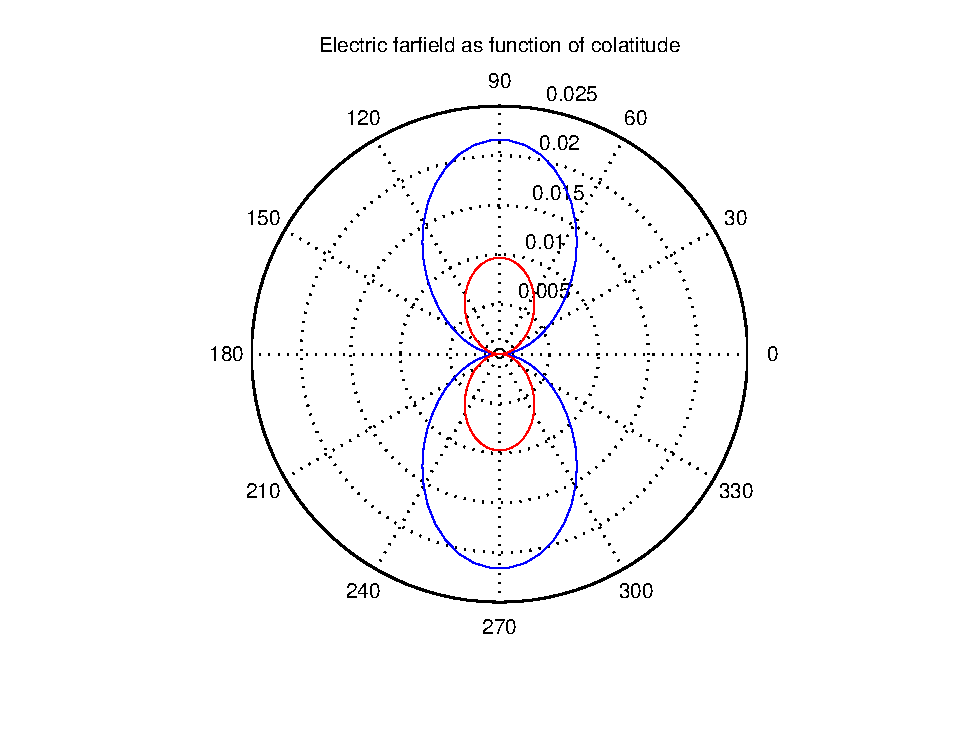
\includegraphics[width=20pc]{ff_10mhz.eps}
\caption{Electric far-field-patterns for the 6m dipole in vacuum (blue) and in plasma (red), computed with solver 2.}
\label{fig:patterns_vacuum}
\end{figure}

Figure \ref{fig:patterns_vacuum} shows 2-dimensional plots of the electric far-field pattern of the 6m dipole at $10 MHz$ in vacuum (upper figure) and in isotropic cold plasma, using a relative permittivity of 0.5. The result is in perfect agreement with the results when computed with Concept II and with theory. The radiated field in plasma is lower than in vacuum. In this configuration the difference is approximately 1 order of magnitude. The reason is that the antenna current has a smaller magnitude in plasma. This can be understood when considering the governing equation (i.e. Pocklington's equation). The impedance of the medium $\eta$ is lager than in vacuum, which means that the mutual impedances between the wire elements, which are the elements of the matrix in the MoM, are larger in plasma. Hence a smaller current as source produces the required electric field. With physical reasoning the phenomenon of smaller current amplitudes can be understood by realizing that the radiated power density is also proportional to the impedance of the medium. Hence, smaller current amplitudes are demanded by the requirement of energy conservation.\\ 

In this case only electrons are considered. When considering also ions, the magnitude of the respective values of the pattern is even lower by a small amount. The difference is so small that the effect of the ions can be neglected in this case.

\subsection{The effective length vectors}
A very useful antenna property which describes the behavior of a transmitting antenna is the effective length vector. It can be computed as

\begin{equation}\label{eq:heff}
\textbf{h}_{eff}=\frac{1}{I}\int \mathbf{J}(\mathbf{r}')e^{\imath \mathbf{k} \cdot \mathbf{r}'} dV'
 \end{equation}

$I$ is the feed current. In general it is complex and depends upon direction of the incident wave. These dependencies can safely be neglected at low frequencies, i.e. the quasistatic range, where the effective length vector can be regarded as real and constant. This range can be estimated for spacecraft to exist up to frequencies where the wavelength can still be regarded as large in relation to the spacecraft and antenna dimensions. It is a well-known result of antenna theory, that the effective lengths of an ideal dipole is half its physical length. Real antennas, especially spacecraft antennas behave slightly different. The reasons for this deviation from ideal conditions can be found in the shape of the spacecraft body, the base capacitances, the finite diameter of a real antenna, and, as will be shown below, the surrounding space plasma.\\

When using computed effective length vectors for analyzing data, one should keep in mind that they are results of calculating transmitting antennas. In vacuum they can be used to describe receiption properties of antennas due to the principle of reciprocity. This principle is not directly valid in a plasma environment, so the meaning of the effective length vector in plasma has to be investigated.\\


\begin{table}
\caption{Effective length vectors in vacuum [m]}
\label{tab:heff_vacuum}
\begin{tabular}{|c|c|c|c|}
 \hline
 & solver 1  & solver 2  & Concept II \\
\hline
$300 kHz$ & 2.842 & 2.864 & 2.812 \\
$1 MHz$ & 2.843 & 2.866 &  2.813 \\
$10 MHz$ & 2.985 & 3.010 &  2.863  \\
\hline
\end{tabular}
\end{table}

\begin{table}
\caption{Effective length vectors in plasma [m]}
\label{tab:heff_plasma}
\begin{tabular}{|c|c|c|c|}
 \hline
 & solver 1  & solver 2  & Concept II \\
\hline
$300 kHz$ & 2.842 & 2.864 & 2.812  \\
$1 MHz$ & 2.842 & 2.865 & 2.812  \\
$10 MHz$ & 2.912 & 2.935 & 2.789 \\
\hline
\end{tabular}
\end{table}

Tables \ref{tab:heff_vacuum} and \ref{tab:heff_plasma} show the magnitude of the effective length vectors, also called the effective lengths, of the dipole under the specified conditions. The direction of the wave was always taken to be the positive x-axis, i.e. perpendicular to the dipole. Investigations have shown that the directional variation of the effective length vector is only very small at those frequencies used for the calculations.\\

Only the real part is presented here. Since the current is parallel to the z-axis throughout the whole dipole, also the effective length vector is parallel to the z-axis in accordance with (\ref{eq:heff}).\\

As it can be seen, the effect of the plasma is a shortening of the effective length vectors. Although the effect is quite small in the presented data, as well as under most realistic conditions, it is generally true.\\

In the stable frequency range, the relation between the equivalent permittivity and the length of the effective length vector is nearly linear for a dipole. For more complex structures, like real spacecraft, this is not generally true. The proportionality factor for the near-linear behavior depends on the frequency. Figure \ref{fig:relative_heff_shortening} shows the equivalent length of the effective length vector as a function of equivalent permittivity for 3 frequencies. The calculation was performed with solver 2 and Concept II. It can clearly be seen that the most prominent effect of the isotropic plasma on the effective length vector is at the highest frequency.\\

\begin{figure}
  \noindent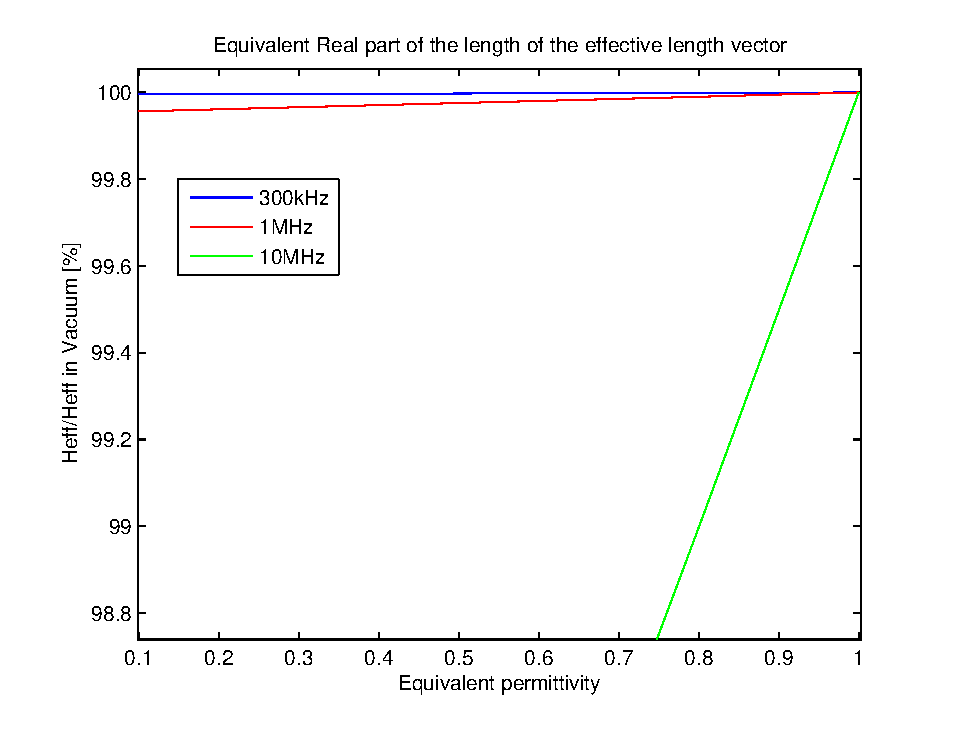
\includegraphics[width=20pc]{heff_shortening_dipole.eps}
\caption{Equivalent length of the effective length vector in relation of vacuum case, as a function of equivalent permittivity.}
\label{fig:relative_heff_shortening}
\end{figure}

\subsection{Impedance patterns}
Figures \ref{fig:impedances_dipole_solver2_real} and \ref{fig:impedances_dipole_solver2_imag} show the real and the imaginary parts of the antenna impedances as a function of frequency. The frequency range is from $100kHz$ to $100MHz$. The results of the calculation for vacuum are plotted in blue, while the plasma case is plotted in red. For these two Figures a constant equivalent permittivity of 0.5 was used. This situation is unrealistic, but we only want to demonstrate the effect of the plasma in the numerical simulation.\\

As it can be seen, the antenna resonances, the frequencies where the imaginary part of the impedance vanishes, are shifted to a higher frequency This corresponds to the effect to be expected for a shorter effective length vector. The plasma effect increases with increasing frequency.\\

Knowledge of the antenna resonances is of vital importance for the correct interpretation of measured data of radio experiments on spacecraft. Especially the even numbered resonances where the imaginary part of the impedance crosses the zero line from the positive to the negative area corresponds to a peak of the curve of the real part and in vicinity of this peak the effective length vectors computed by numerical means can not be considered as reliable since slight variation of the geometry may change the pattern completely. Therefore the inclusion of the plasma effect in numerical calibration can be considered as important, also at radio frequencies.\\


\begin{figure}
  \noindent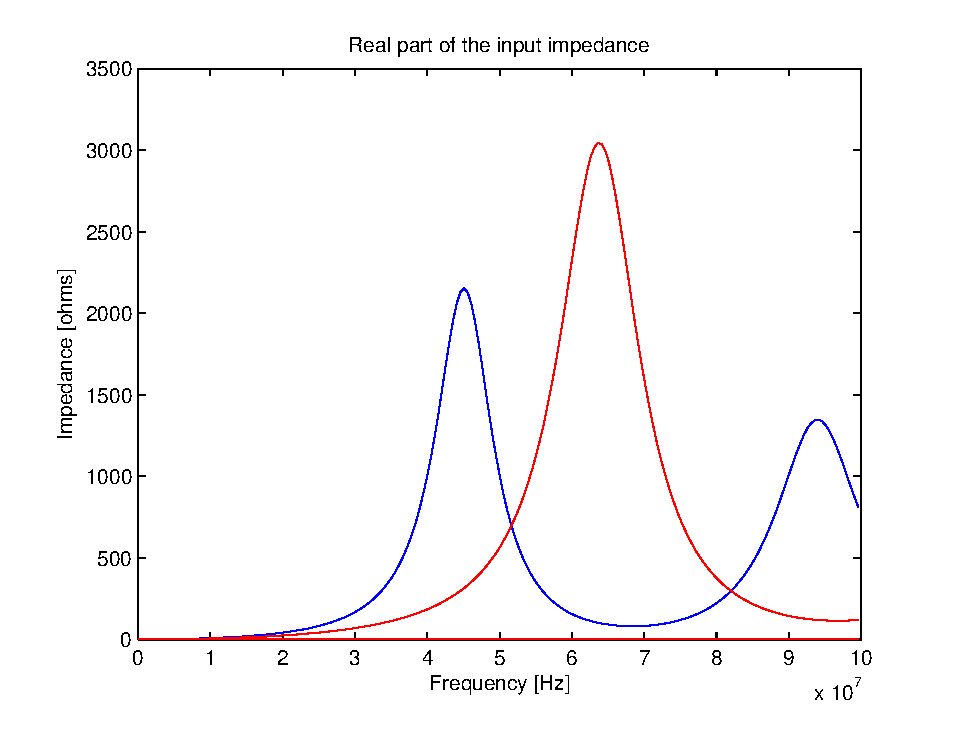
\includegraphics[width=20pc]{imps_dipole_solver2_real.eps}
\caption{Real part of 6m dipole impedance, from $0.1 - 100 MHz$, computed with solver 2. The blue line shows the impedance in vacuum, whereas for the red line $\epsilon_r$ was held constant at $0.5$.}
\label{fig:impedances_dipole_solver2_real}
\end{figure}

\begin{figure}
\noindent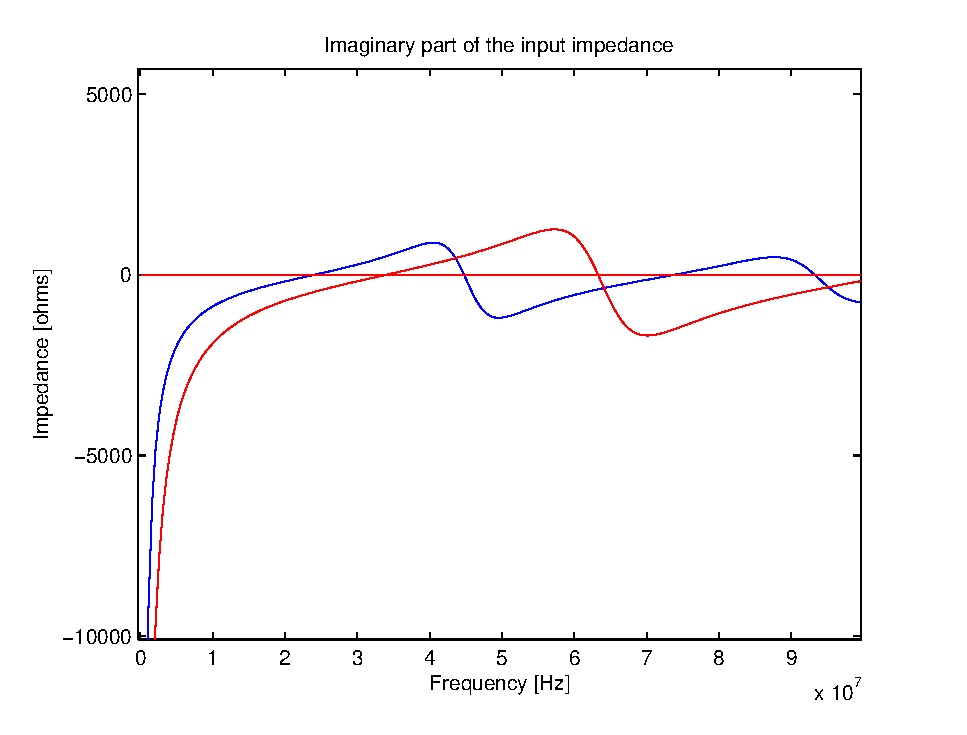
\includegraphics[width=20pc]{imps_dipole_solver2_imag.eps}
\caption{Imaginary part of 6m dipole impedance, from $0.1 - 100 MHz$, computed with solver 2. The blue line shows the impedance in vacuum, whereas for the red line $\epsilon_r$ was held constant at $0.5$.}
\label{fig:impedances_dipole_solver2_imag}
\end{figure}

The realistic case is more subtle. Figures \ref{fig:impedances_dipole_solver2_2_real} and \ref{fig:impedances_dipole_solver2_2_imag} show a similar calculation, but this time the plasma electron frequency was set to $10MHz$, a situation which could be realistic in some dense plasma environments in space, as in the ionosphere. The frequency range in these figures is from $10.1$ to $100MHz$. The differences between vacuum and plasma are smaller and decrease with higher frequency. The electron plasma frequency is a cutoff, where the imaginary part of the antenna impedance tends to minus infinity and no electromagnetic radio waves can propagate.

\begin{figure}
  \noindent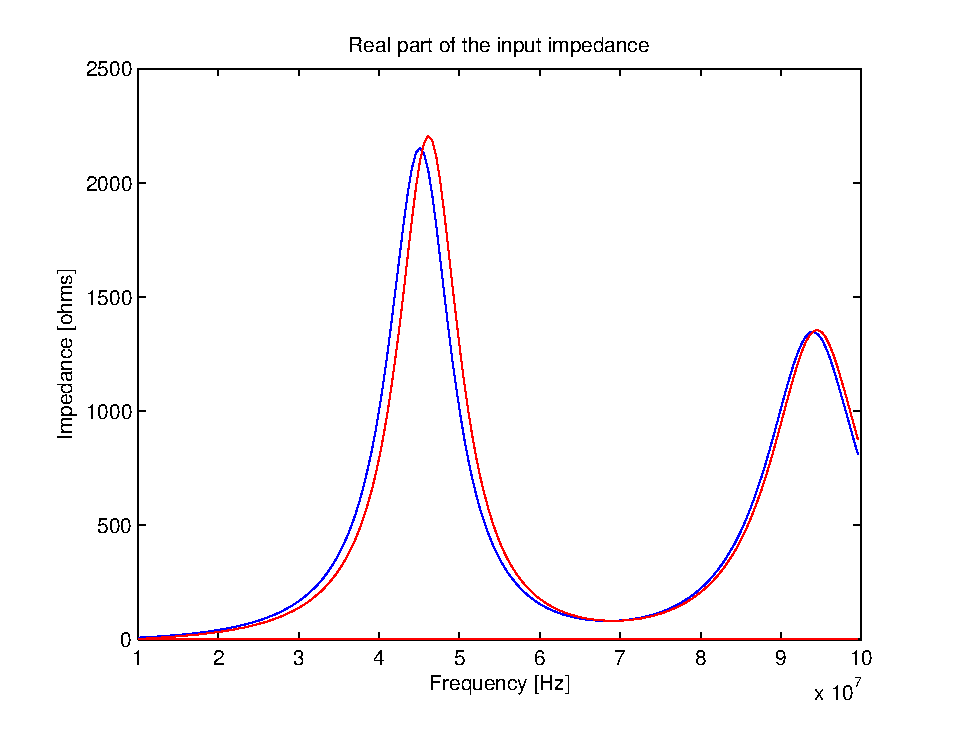
\includegraphics[width=20pc]{imps_dipole_solver2_real2.eps}
\caption{Real part of antenna impedance, $10.1 - 100 MHz$, computed with solver 2. $f_p=10MHz$. The blue line shows the impedance in vacuum, whereas the red line is the plasma solution.}
\label{fig:impedances_dipole_solver2_2_real}
\end{figure}

\begin{figure}
\noindent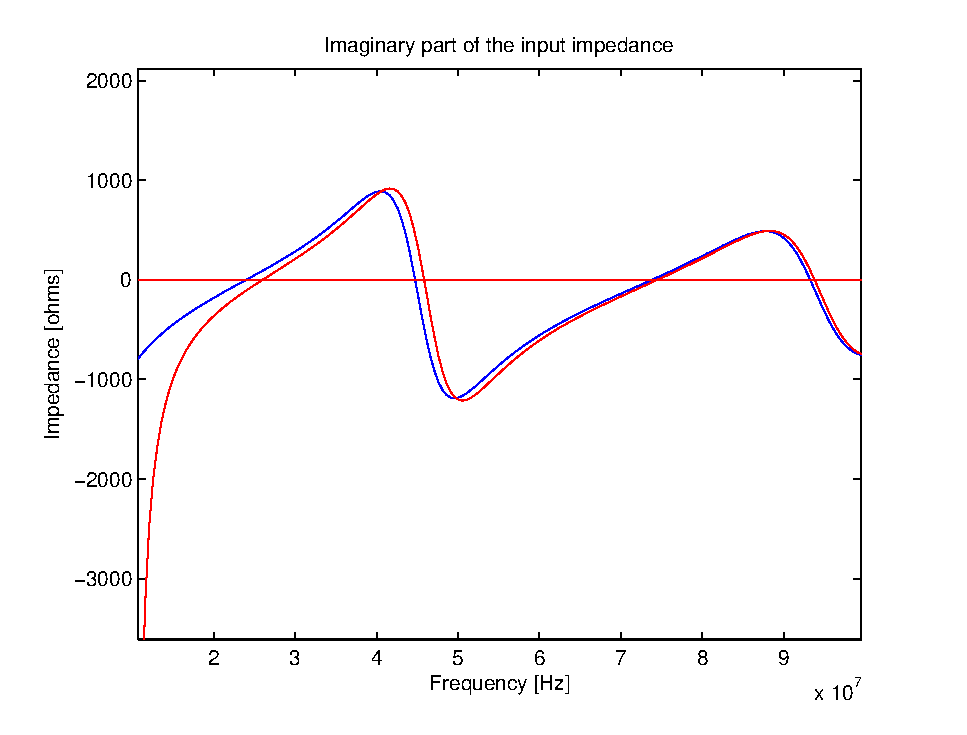
\includegraphics[width=20pc]{imps_dipole_solver2_imag2.eps}
\caption{Imaginary part of antenna impedance, $10.1 - 100 MHz$, computed with solver 2. $f_p=10MHz$. The blue line shows the impedance in vacuum, whereas the red line is the plasma solution.}
\label{fig:impedances_dipole_solver2_2_imag}
\end{figure}

\section{Application to a real spacecraft (STEREO)}
In this section the effect of space plasma will be included in the calculation of antenna properties of actual spacecraft antennas.\\

The spacecraft upon which the calculations are applied is the STEREO A spacecraft. The reason for this is that there exists a good wire and patch model as well as experimental results and actual measured data. Additionally the authors of this paper have some experience with regard to antenna calibration with this spacecraft (\cite{ossi09} and \cite{panchenko10}). The respective wire/patch grid model is shown in Figure \ref{fig:stereo}.\\

\subsection{The STEREO mission and the WAVES experiment}
On October $25^{th}$, 2006, NASA launched the two STEREO spacecraft with a radio experiment on board, called STEREO-WAVES (S/WAVES), which is designed to observe solar radio emissions by using direction finding capabilities. The S/WAVES experiment is designed to track solar and interplanetary radio bursts and trace the generation and evolution of radio disturbances from the Sun to Earth orbit and beyond. Each spacecraft has three orthogonal antennas, capable of receiving electromagnetic waves in several frequency ranges. The main operational range of the receivers is between 10kHz and 16MHz. With this configuration, it is possible to perform goniopolarimetry at the lower end of the frequency range to determine the direction of incidence and the polarization of the received radiation. When both spacecraft receive radiation from the same source, the actual location of the source can be pinpointed by the method of triangulation.\\

For the correct interpretation of the data it is of vital importance to know the antenna properties with great accuracy. Numerical and experimental antenna calibration was performed by the Radio Group of the Space Research Institute of the Austrian Academy of Sciences, based in Graz. During these calibrations, which are published in \cite{ossi09} and \cite{macher07} a vacuum environment was postulated. In this section the effect of an isotropic plasma on the results of the numerical calibration will be discussed.\\

\begin{figure*}
\noindent\includegraphics[width=39pc]{stereo.eps}
  \caption{The STEREO spacecraft wiregrid.}\label{fig:stereo}
\end{figure*}

The STEREO/WAVES experiment works with three mutually orthogonal stacer
monopole antennas. This paper applies to the HFR and band B and C of the LFR. The HFR operates in a range from 125 kHz to 16.025 MHz. The HFR provides all auto- and cross-correlation parameters. Two direction finding (DF) modes are implemented, one of which uses the antennas as dipoles. The other DF mode uses the antennas as monopoles. The HFR is a sweeping frequency receiver and each sweep takes approximately 15 seconds. Only the monopoles are treated in this article.\\

Bands B and C provide auto- and cross-correlation parameters and can be used
for DF.\\
\subsection{The effect on the antenna impedances}

\begin{figure}
 \noindent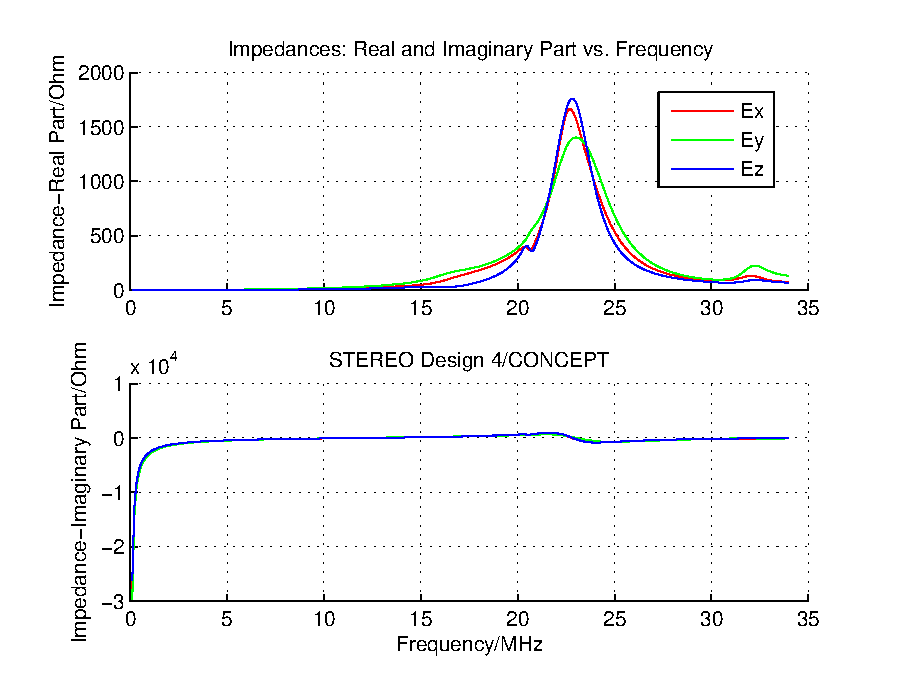
\includegraphics[width=20pc]{impedance_stereo_vac.eps}
  \caption{The impedance of the S/WAVES antennas in vacuum.}\label{fig:imp_stereo_real}
\end{figure}

\begin{figure}
\noindent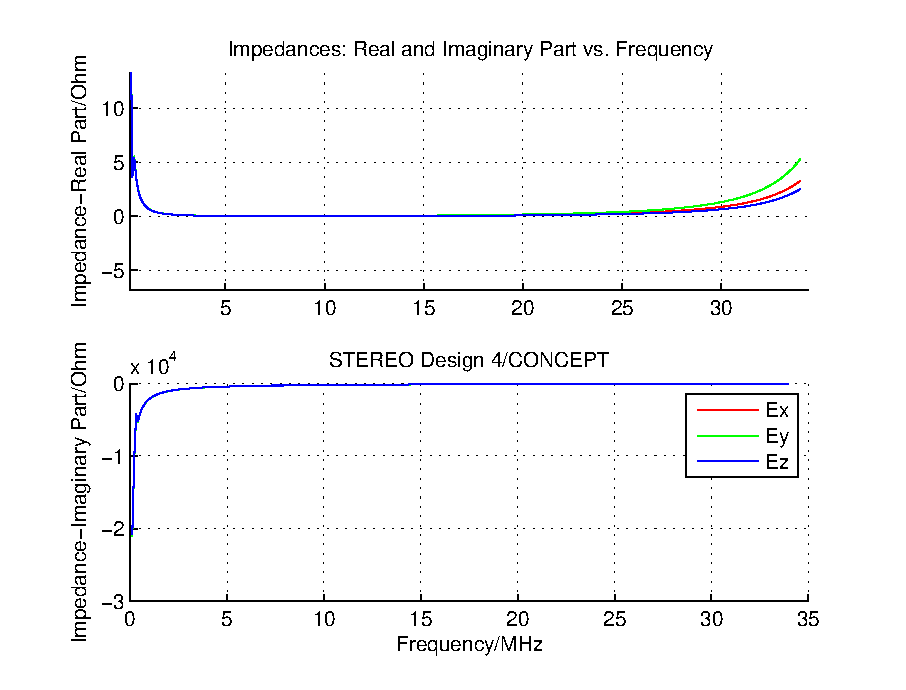
\includegraphics[width=20pc]{impedance_stereo_pl.eps}
  \caption{The impedance of the S/WAVES antennas in cold plasma with $\epsilon_r=0.1$.}\label{fig:imp_stereo_imag}
\end{figure}

Figures \ref{fig:imp_stereo_real} and \ref{fig:imp_stereo_imag} show the results of these calculations, performed with a constant equivalent permittivity of $0.1$, again for demonstration purposes. The effect on the impedance curve shows the same behavior as for the dipole. The resonance is shifted to a higher frequency. The curves for the three antennas are so close together at some parts, that they appear as single line.\\

\begin{figure}
\noindent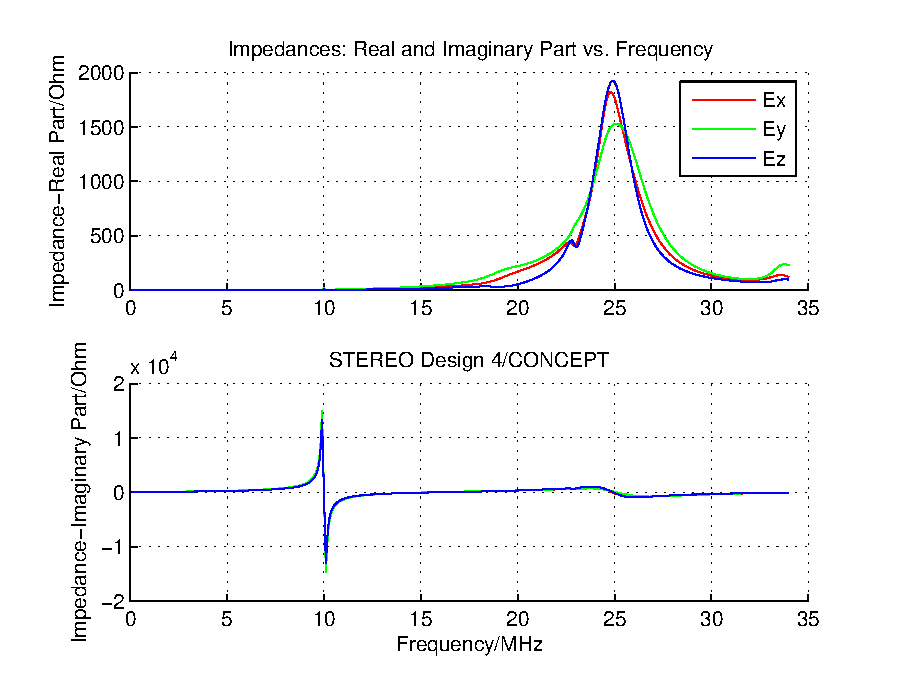
\includegraphics[width=20pc]{impedance_stereo_pl_fix.eps}
  \caption{The impedance of the S/WAVES antennas in cold plasma with $f_{pe}=10MHz$.}\label{fig:imp_stereo_fix}
\end{figure}

Figures \ref{fig:imp_stereo_fix} show the same calculation with a fixed electron plasma frequency of 10MHz. Only the part of the graph above 10MHz is relevant. The calculation is not valid at the lower frequency range.\\

One can see the shift of the second antenna resonance due to the influence of the plasma. Even on the realistic plot with the fixed plasma frequency, the peak of the real part of the impedance curve is shifted by more than 2 MHz. STEREO will not have to deal with conditions where such high plasma frequencies exist, but for other space missions taking measurements inside the ionosphere, or, although with lower resonance frequencies, in planetary magnetospheres, such shifts should be take into account.\\

The plasma frequency is

\begin{equation}\label{Plasma frequency}
    f_p=\sqrt{\frac{1}{2\pi}{\frac{n_e e^2}{ m \epsilon_0}}}
\end{equation}

At conditions where STEREO operates, i.e. at 1AU in interplanetary space, which corresponds roughly to an electron plasma frequency between 20kHz and 60kHz, we will set the electron plasma frequency to a rounded value of 100kHz. Figure \ref{fig:imp_stereo_fix_100kHz} shows the result. To the resolution of this figure, there is no visible difference to the vacuum computation. Hence, it seems that the plasma effect can be neglected for the calculation of the impedance curves and the estimation of the antenna resonances of the radio experiment of the STEREO spacecraft.


\begin{figure}
\noindent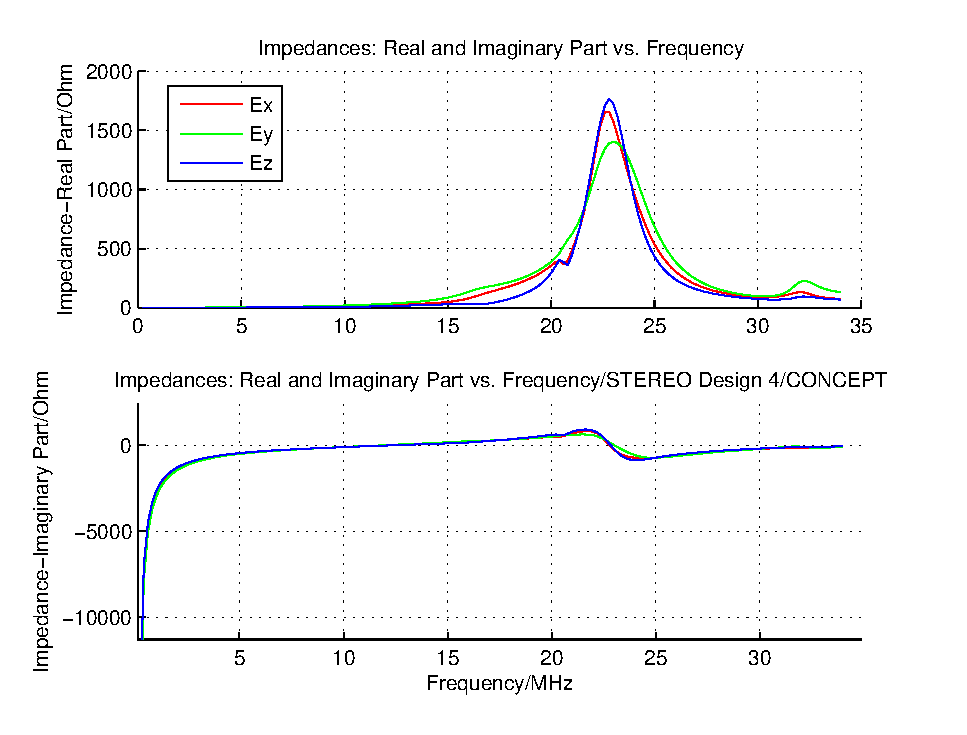
\includegraphics[width=20pc]{impedance_stereo_pl_100khz.eps}
  \caption{The impedance of the S/WAVES antennas in cold plasma with $f_{pe}=100kHz$.}\label{fig:imp_stereo_fix_100kHz}
\end{figure}

\subsection{The effect on the effective length vectors}
Computing the effective length vectors using the cold plasma permittivity results in a slightly shorter effective length vector. The directions are not altered very much. As an example the quasistatic effective length vectors of the STEREO antennas are given in Tables \ref{tab:heff_vacuum_stereo} and \ref{tab:heff_cold_plasma_stereo}. In both cases a frequency of $300kHz$ is used, which is a typical value when investigating the behavior of an antenna in the quasistatic limit. At the first table, vacuum is used as the surrounding medium, while a cold isotropic plasma model is used for comparison (Table \ref{tab:heff_cold_plasma_stereo}), using again the realistic value of 100kHz as electron plasma frequency.\\

Plasma frequency and wave frequency are close together in this example, so the difference in length of the effective length vectors is clearly visible (about 10cm) and should be considered for data processing of the measured S/WAVES data.

The coordinate frame used for presenting the effective lengths vectors is a spherical polar coordinate frame with the principle axes point towards the x-axis, i.e. the direction of the sun. The coordinates of the physical antennas are shown in Table \ref{tab:phys_ant}. Details can be found in \cite{ossi09}. \\

For the calculations, base capacitances of $70pF$ where used. The inclusion of base capacitances has also the effect of decreasing the lengths of the effective length vectors.\\
\begin{table}
\caption{Physical antennas}
\label{tab:phys_ant}
\begin{tabular}{|c|c|c|c|}
 \hline
 & $length/m$ & $\zeta/^\circ$ & $\xi/^\circ$ \\
\hline
$E_x$ & $6.00$ & $125.3$ & $-120.0$ \\
$E_y$ & $6.00$ & $125.3$ & $120.0$ \\
$E_z$ & $6.00$ & $125.3$ & $0.00$ \\
\hline\end{tabular}
\end{table}

\begin{table}
\caption{Effective length vectors in vacuum: $f=300kHz$}
\label{tab:heff_vacuum_stereo}
\begin{tabular}{|c|c|c|c|}
 \hline
 & $length/m$ & $\zeta/^\circ$ & $\xi/^\circ$ \\
\hline
$E_x$ & $1.35$ & $119.9$ & $-135.3$ \\
$E_y$ & $1.64$ & $114.4$ & $127.3$ \\
$E_z$ & $1.09$ & $124.7$ & $15.5$ \\
\hline\end{tabular}
\end{table}



\begin{table}
\caption{Effective length vectors in cold plasma: f=300kHz, $f_{pe}=100kHz$}
\label{tab:heff_cold_plasma_stereo}
\begin{tabular}{|c|c|c|c|}
 \hline
 & $length/m$ & $\zeta/^\circ$ & $\xi/^\circ$ \\
\hline
$E_x$ & $1.26$ & $119.6$ & $-135.0$ \\
$E_y$ & $1.53$ & $114.1$ & $127.2$ \\
$E_z$ & $1.02$ & $124.3$ & $15.2$ \\
\hline\end{tabular}
\end{table}



\begin{figure}
  \noindent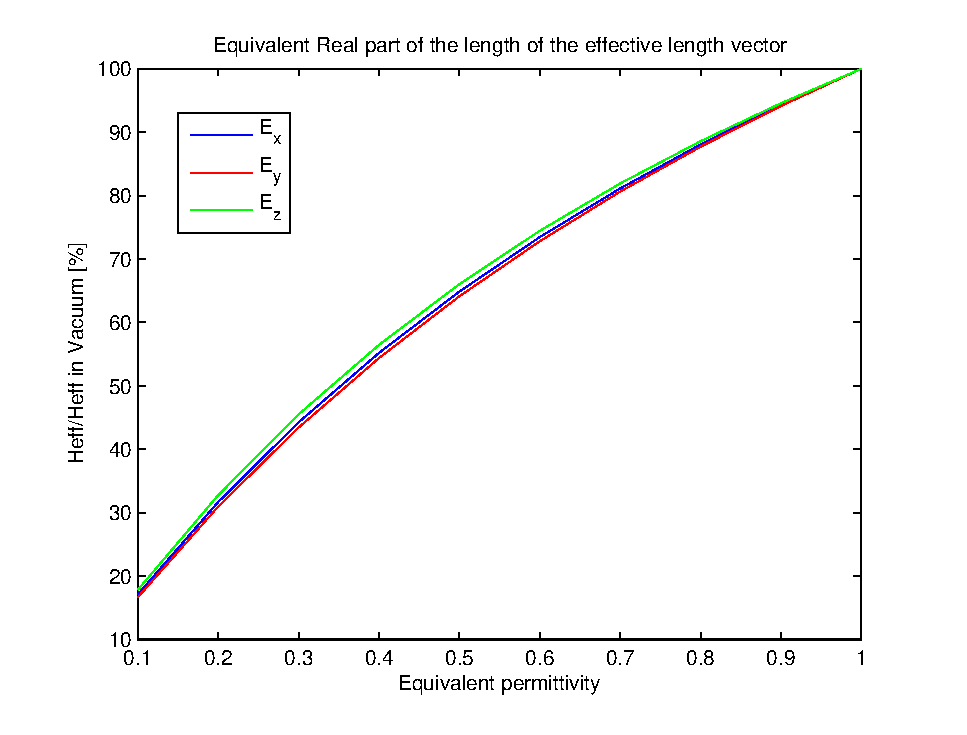
\includegraphics[width=20pc]{heff_shortening_stereo.eps}
\caption{Equivalent length of the effective length vector in relation of vacuum case, as a function of equivalent permittivity.}
\label{fig:relative_heff_shortening_stereo}
\end{figure}

Figure \ref{fig:relative_heff_shortening_stereo} shows the equivalent reduction of the length of the effective length vector in relation to the vacuum case as a function of the equivalent permittivity for all three STEREO/WAVES antennas at a frequency of 300kHz. It can be seen that the relative shortening is far more pronounced than for the dipole. This graph can be used to estimate the plasma effect on the effective length vectors for calibration purposes. Similar figures can easily be produced for a selection of frequencies.\\

\section{Conclusion}
In this article, the effect of plasma on spacecraft antenna properties was investigated. On a theoretical basis a method was shown, how the plasma effect can be incorporated into numerical antenna calibration. It was also shown that a simple model of cold plasma is valid for this task. Kinetic, relativistic or quantum mechanical treatment is not necessary.\\

Two simple solvers were implemented, using a boundary element method known as Method of Moments, to solve the electric field integral equation for computing the current distribution along a dipole. For validation, the results where compared to the results of 2 well proven solvers, one open source software called ASAP, and one proprietary program, called Concept II.\\

Using these solvers, simple calculations of antennas in isotropic plasma where performed and studied. Then calculations where performed for antennas of a real space radio experiment, S/WAVES mounted on the STEREO spacecraft. It was shown that the effects of the plasma in interplanetary space at approximately 1AU, i.e. the regime where STEREO operates, are so small they can be neglected for certain applications. The effect of the the plasma on the effective length vectors in the quasistatic range is present, however (approximately 10cm) and should be considered for data interpretation. For space missions operating in different regimes, especially in the ionosphere, the effect of plasma on the antenna properties in the radio frequency range could be more dramatic, which make a careful analysis mandatory.\\


%% ------------------------------------------------------------------------ %%
%
%  TEXT
%
%% ------------------------------------------------------------------------ %%



%%% End of body of article:

%%%%%%%%%%%%%%%%%%%%%%%%%%%%%%%%
%% Optional Appendix goes here
%
%%%%%%%%%%%%%%%%%
% Geophysical Research Letters only allows an appendix without a letter.
%% You can get this result with
%  \section*{Appendix}
%  or
%  \section*{Appendix: Title}
%%%%%%%%%%%%%%%%%
%
% \appendix resets counters and redefines section heads
% but doesn't print anything.
% After typing  \appendix
%
% \section{Here Is Appendix Title}
% will print
% Appendix A: Here Is Appendix Title
%
% \section*{Appendix}
% will print
% Appendix
%
% \section*{Appendix: Here Is Appendix Title}
% will print
% Appendix: Here Is Appendix Title
%
% For only 1 appendix \appendix \section{Appendix} is preferred.
% which will print
% Appendix A

%%%%%%%%%%%%%%%%%%%%%%%%%%%%%%%%%%%%%%%%%%%%%%%%%%%%%%%%%%%%%%%%
%
% Optional Glossary or Notation section, goes here
%
%%%%%%%%%%%%%%
% Glossary only allowed in Reviews of Geophysics
% \section*{Glossary}
% \paragraph{Term}
% Term Definition here
%
%%%%%%%%%%%%%%
% Notation -- End each entry with a period.
% \begin{notation}
% Term & definition.\\
% Second Term & second definition.
% \end{notation}
%%%%%%%%%%%%%%%%%%%%%%%%%%%%%%%%%%%%%%%%%%%%%%%%%%%%%%%%%%%%%%%%
%
%  ACKNOWLEDGMENTS

\begin{acknowledgments}
The authors want to thank the members of the STEREO/WAVES team for the support and for sharing the necessary data to perform the studies which led to this article.
\end{acknowledgments}

%% ------------------------------------------------------------------------ %%
%
%  REFERENCE LIST AND TEXT CITATIONS
%
% Either type in your references using
% \begin{thebibliography}{}
% \bibitem{}
% Text
% \end{thebibliography}
%
% Or,
%
% If you use BiBTeX for your References, please produce your .bbl
% file and copy the contents into your paper here.
%
% Follow these steps:
% 1. Run LaTeX on your LaTeX file.
%
% 2. Run BiBTeX on your LaTeX file.
%
% 3. Open the new .bbl file containing the reference list and
%   copy all the contents into your LaTeX file here.
%
% 4. Comment out the old \bibliographystyle and \bibliography commands.
%
% 5. Run LaTeX on your new file before submitting.
%
% AGU does not want a .bib or a .bbl file, but asks that you
% copy in the contents of your .bbl file here.

\begin{thebibliography}{}
\bibitem[{\textit{Davidson}(2005)}]{davidson}
Davidson, B. (2005), \textit{Computational Electromagnetics for RF and
  Mictrowave Engineering}, Cambridge University Press.

\bibitem[{\textit{Ginzburg}(1970)}]{ginzburg}
Ginzburg, V. (1970), \textit{The propagation of electromagnetic waves in
  plasma, Second Edition}, Pergamon Press.

\bibitem[{\textit{Harrington}(1968)}]{harrington}
Harrington, R. (1968), \textit{Field Computation by Moment Methods}, Robert E.
  Krieger Publishing Company.

\bibitem[{\textit{Macher et~al.}(2007)\textit{Macher, Oswald, Fischer, and
  Rucker}}]{macher07}
Macher, W., T.~Oswald, G.~Fischer, and H.~Rucker (2007), Rheometry of
  multi-port spaceborn antennas including mutual antenna capacitances and
  application to stereo/waves., \textit{Meas. Sci. Technol.}, \textit{18},
  3731--3742.

\bibitem[{\textit{Melrose}(1980)}]{melrose1}
Melrose, D. (1980), \textit{Plasma Astrophysics: Nonthermal Processes in
  Diffuse Magnetized Plasma}, Gordon and Beach Science Publishers.

\bibitem[{\textit{Oswald et~al.}(2009)\textit{Oswald, Macher, Rucker, Fischer,
  Taubenschuss, Bougeret, Lecacheux, Kaiser, and Goetz}}]{ossi09}
Oswald, T., W.~Macher, H.~Rucker, G.~Fischer, U.~Taubenschuss, J.~Bougeret,
  A.~Lecacheux, M.~Kaiser, and K.~Goetz (2009), Various methods of calibration
  of the stereo/waves antennas, \textit{Adv. Space Res.},\textit{43},
  355--364.

\bibitem[{\textit{Panchenko et~al.}(2010)\textit{Panchenko, Rucker, Macher,
  Cecconi, Oswald, and Fischer}}]{panchenko10}
Panchenko, M., H.~Rucker, W.~Macher, B.~Cecconi, T.~Oswald, and G.~Fischer
  (2010), Stereo/waves antennas calibrated by akr, in \textit{European
  Planetary Science Congress 2010}, vol.~5.

\bibitem[{\textit{Richmond}(1966)}]{richmond66}
Richmond, J. (1966), A wire-grid model for scattering by conducting bodies,
  \textit{IEEE Transactions on Antennes and Propagation}, \textit{14},
  782--786.

\bibitem[{\textit{Stix}(1992)}]{stix}
Stix, T. (1992), \textit{Waves in Plasmas}, American Institute of Physics.



\end{thebibliography}


\end{article}



\end{document}

